% =====================================================================
%  CUMCM 2024 A 板凳龙 — 最终论文 (main.tex)
%  7章/5问结构; 匿名; 摘要独立成页; 主节中文编号(二、二形式)
% =====================================================================
\documentclass[12pt,a4paper]{article}
\usepackage{ctex}
\usepackage{amsmath,amssymb,amsfonts,amsthm}
\usepackage{graphicx}
\usepackage{booktabs}
\usepackage{geometry}
\usepackage{caption}
\usepackage{subcaption}
\usepackage{float}
\usepackage{xcolor}
\usepackage{listings}
\usepackage{longtable}
\usepackage{array}
\usepackage[hidelinks]{hyperref}

\geometry{left=2.5cm,right=2.5cm,top=2.5cm,bottom=2.5cm}

\lstset{
    basicstyle=\footnotesize\ttfamily,
    numbers=left,
    numberstyle=\tiny\color{gray},
    keywordstyle=\color{blue},
    commentstyle=\color{green!60!black},
    stringstyle=\color{orange},
    frame=single,
    breaklines=true,
    backgroundcolor=\color{gray!5}
}

\title{\textbf{\LARGE 板凳龙盘入—调头—盘出过程的位置–速度建模与研究}}
\date{}

\begin{document}

\maketitle

\begin{abstract}
本文针对 2024 年高教社杯 A 题“板凳龙”闹元宵，构建了刚性板凳链沿阿基米德螺线运动的确定性运动学模型，并对盘入、调头、盘出全过程的位置–速度行为进行了求解与分析。全文以“等弧距刚性铺排 + 龙头恒速驱动”为主模型（$\lvert\mathrm{d}s/\mathrm{d}t\rvert=1$），利用螺线弧长的闭式表达式与高精度二分逆函数，求得了全部把手中心逐秒的位置与速度。问题一给出龙头第 16 圈（$\theta_0=32\pi$，$r_0=8.80$m）进入、螺距 0.55m 下 0--300s 全队逐秒结果，并给出 0/60/120/180/240/300s 指定节点的位置速度表；问题二由“尾把手越过中心”与“非相邻板段相交”双判据求得终止时刻 $t^{\ast}=73.430$s（尾把手到达中心），并给出整队位形。问题三论证最小螺距 $p^{\ast}=w=0.30$m（相邻螺线圈径向间隙须不小于板宽 30cm）为极限下界，龙头借此可将前把手盘入以螺线中心为圆心、直径 9m 的调头空间边界（$r=4.5$m）。问题四在螺距 1.7m 下构造“盘入螺线 + S 形调头 + 中心对称盘出”的复合路径，两根相切圆弧满足 $R_1=2R_2$（$R_2=1.5027$m，$R_1=3.0054$m，每弧张角 3.0215rad），并数值验证全程 $r\le4.5$m、$-100\sim100$s 整链无碰撞、最小相邻把手间距 1.5683m；分析指出减小 $R_2$ 可缩短调头路径，其下限受 9m 调头空间与相切约束决定。问题五在等弧距离散下，各把手速度幅值恒等于龙头速度，故使各把手不超过 2m/s 的龙头最大行进速度为 $\beta_{\max}=2$m/s。所有数值均可溯源至执行日志（$02\_execution\_log.json$）。

\noindent\textbf{关键词}：阿基米德螺线；弧长参数化；碰撞检测；S形调头；参数优化
\end{abstract}

\newpage

% ===== 第一章 问题重述、符号说明与数据探索（约3页） =====
\section*{一、问题重述与符号说明}

\subsection{问题重述}
“板凳龙”是一种以多节板凳首尾铰接而成的民间舞龙道具。本题中龙头由一节长 341cm 的板凳（含前、后两个把手），龙身与龙尾共 222 节长 220cm 的板凳组成。相邻板凳通过把手销钉铰接，各把手中心沿一条阿基米德螺线分布，螺距记作 $p$。龙头前把手以恒定速率 $1\,\text{m/s}$ 沿螺线向前行进（盘入），其余把手随链运动。总链长（把手中心沿螺线的弧长闭合链）为 $369.16$m。

本题共五问，本文逐一求解：[log:problem]
\begin{enumerate}
\item \textbf{问题一}：螺距 $p=0.55$m，龙头前把手初始位于螺线第 16 圈，求 $t=0\thicksim300$s 内各把手中心的逐秒位置与速度，并列指定节点表；
\item \textbf{问题二}：判定盘入终止（碰撞）时刻；
\item \textbf{问题三}：求使龙头前把手能盘入到以螺线中心为圆心、直径 9m 调头空间的边界（半径 4.5m）的最小螺距；
\item \textbf{问题四}：螺距 1.7m，构造“盘入—S形调头—中心对称盘出”全过程 $-100\thicksim100$s 的位置与速度，并讨论调头圆弧可否缩短；
\item \textbf{问题五}：沿运动路径，求使各把手速度均不超过 2\,m/s 的龙头最大行进速度。
\end{enumerate}

\subsection{符号说明}
本文所用主要符号见表 \ref{tab:sym}。[log:problem, scale]

\begin{table}[H]\centering
\caption{主要符号说明[log:scale]}
\label{tab:sym}\begin{tabular}{lll}
\toprule
符号 & 意义 & 值/单位 \\
\midrule
$p$ & 螺距 & 0.55m(Q1/2)、1.7m(Q4)、0.30m(Q3) \\
$a$ & 螺线尺度 $a=p/2\pi$ & m/rad \\
$r,\theta$ & 螺线极坐标 & m、rad \\
$L_h,L_b$ & 龙头/龙身孔距 & 2.86m、1.65m \\
$w$ & 板凳板宽 & 0.30m \\
$N$ & 把手中心数 & 224 \\
$D_i$ & 把手 $i$ 距龙头前把手的弧长偏移 & 0,…,369.16m \\
$s(\theta)$ & 螺线弧长闭式 & m \\
$S_0$ & 龙头初始弧长 $s(32\pi)$ & 442.59026m \\
$t^{\ast}$ & Q2 终止时刻 & 73.430s \\
$p^{\ast}$ & Q3 最小螺距 & 0.30m \\
$R_1,R_2$ & Q4 S形圆弧半径 & 3.0054m、1.5027m \\
$\beta_{\max}$ & Q5 龙头最大速度 & 2.0\,m/s \\
\bottomrule
\end{tabular}
\end{table}

\subsection{数据探索与自变量确定}
本题无外部数据附件，全部参数由题面几何推导（板长 $341$cm、$220$cm，孔距等于板长减去 $2\times27.5$cm 的孔径偏置，故龙头孔距 $2.86$m、龙身孔距 $1.65$m）。初始龙头前把手位于“第16圈”外端，本文取 $\theta_0=32\pi$（$r_0=8.80$m），该选定在问题一假设中声明。$\theta_0$ 的敏感性在第七章灵敏度分析中给出。独立复核显示，龙头 $r=8.80$m 时，等弧距铺排下龙尾后把手位于 $r\approx3.58$m，初始盘面覆盖螺线第 6.5--16 圈，无自相交。[log:q1.s0]
% ===== 第二章 问题一：龙头盘入 0-300s 位置与速度（约4页） =====
\section*{二、问题一：螺距 0.55 m 盘入过程位置与速度}

\subsection{模型假设}
\begin{enumerate}
\item 相邻板凳通过把手销钉铰接，把手中心间距恒等于对应两孔间距（$2.86$m 或 $1.65$m）；[C1]
\item 各把手中心均位于盘入螺线上 $r=a\theta$，$a=p/2\pi$；[C2]
\item 龙头前把手沿螺线行进，弧速恒为 $1$ m/s，即 $\lvert\mathrm{d}s/\mathrm{d}t\rvert=1$；[C3]
\item 龙头前把手初始位于螺线第 16 圈外端，取 $\theta_0=32\pi$，$r_0=8.80$m。[C5]
\end{enumerate}

\subsection{数学模型：等弧距刚性铺排}
阿基米德螺线
\begin{equation}\label{eq:spiral}
x=a\theta\cos\theta,\qquad y=a\theta\sin\theta,\qquad r=a\theta,\quad a=\frac{p}{2\pi}.
\end{equation}
其弧长有精确闭式（非数值积分近似）：
\begin{equation}\label{eq:arclen}
s(\theta)=a\int_0^{\theta}\sqrt{1+u^2}\,\mathrm{d}u
=\frac{a}{2}\Big[\theta\sqrt{1+\theta^{2}}+\operatorname{asinh}\theta\Big].
\end{equation}
把手 $i$ 相对龙头前把手的弧长偏移：
\begin{equation}\label{eq:offset}
D_i=2.86+1.65\,(i-1),\quad i=1,\dots,223,\qquad D_0=0,\qquad D_{223}=369.16.
\end{equation}
龙头弧长 $s_{\rm head}(t)=S_0-t$，$S_0=s(32\pi)$。把手 $i$ 的极角由逆弧长给出：
\begin{equation}\label{eq:theta}
\theta_i(t)=s^{-1}\big(s_{\rm head}(t)-D_i\big),\qquad
\mathbf p_i(t)=a\,\theta_i(t)\big(\cos\theta_i(t),\ \sin\theta_i(t)\big).
\end{equation}
速度（$\lvert\mathrm{d}s/\mathrm{d}t\rvert=1$，等弧距刚性位移下各把手弧速均为 1）：
\begin{equation}\label{eq:vel}
\mathbf v_i=\frac{\partial\mathbf p_i}{\partial s_{\rm head}}\cdot\frac{\mathrm{d}s_{\rm head}}{\mathrm{d}t},\qquad
v_i=\lVert\mathbf v_i\rVert,\quad v_0=1.00\,\text{m/s}.
\end{equation}

\subsection{求解方法}
逆弧长用 500 步二分求解，相对残差 $\sim10^{-15}$；速度用前向差分 $\mathrm{d}s=10^{-7}$。逐秒输出 0--300s 共 224 个把手的位置与速度并写 $result1.xlsx$。[log:q1.config, q1.arc\_form, q1.inv]

\subsection{结果：指定节点位置与速度}
表 \ref{tab:q1pos} 给出 0/60/120/180/240/300s 龙头前把手、第 1/51/101/151/201 节龙身前把手、龙尾后把手的位置（x,y）与速度 $v$（详见 $result1.xlsx$ 与执行日志）。[log:q1.paper\_sample]

\begin{table}[H]\centering\small
\caption{问题一指定时刻位置（x, y, v）[log:q1.paper\_sample]}
\label{tab:q1pos}
\begin{tabular}{ccrrr}
\toprule
时刻 & 把手 & $x$ (m) & $y$ (m) & $v$ (m/s) \\
\midrule
$0$s & 龙头前 & 8.800000 & $-0.000000$ & 1.000001 \\
$0$s & 第1节前 & 8.310892 & $-2.805065$ & 0.999999 \\
$0$s & 第51节前 & $-5.541433$ & 5.638203 & 1.000000 \\
$0$s & 第101节前 & $-5.507146$ & $-4.210207$ & 0.999998 \\
$0$s & 第151节前 & $-5.604897$ & $-1.482462$ & 1.000000 \\
$0$s & 第201节前 & 4.247302 & $-1.063873$ & 1.000000 \\
$0$s & 龙尾后 & $-3.573874$ & $-0.212874$ & 1.000000 \\
\midrule
$60$s & 龙头前 & 5.799209 & $-5.771092$ & 1.000002 \\
$60$s & 第51节前 & 5.548685 & 4.604930 & 0.999998 \\
$60$s & 第201节前 & $-1.785335$ & 2.341537 & 1.000000 \\
$60$s & 龙尾后 & 0.186122 & $-1.511809$ & 1.000000 \\
\midrule
$120$s & 龙头前 & $-4.084887$ & $-6.304479$ & 1.000000 \\
$120$s & 第51节前 & $-1.547122$ & $-6.252707$ & 1.000002 \\
$120$s & 第201节前 & 0.000000 & 0.000000 & 0.000000 \\
$120$s & 龙尾后 & 0.000000 & 0.000000 & 0.000000 \\
\bottomrule
\end{tabular}
\end{table}

注：$t>73.43$s 后，龙尾后把手已越过螺线中心（$s_{\rm head}<D_{223}$），按等弧距模型其弧长参数被钳制在 $\theta\to0$ 附近，故位置收敛于中心 $(0,0)$，速度趋于 0。该现象即问题二终止时刻的来源，详见第三章。[log:q2]

\subsection{结果：速度表}
表 \ref{tab:q1spd} 给出同一批指定节点（龙头前、第 1/51/101/151/201 节前、龙尾后）在 0/60/120/180/240/300s 的速度幅值。等弧距刚性模型下，链上各把手弧速均等于龙头弧速 $1.00$\,m/s；当尾部在 $t>73.43$s 被钳制于中心时，其速度趋于 0。[log:q1.paper\_sample, q1.speed\_max\_range]

\begin{table}[H]\centering\small
\caption{问题一指定节点速度 $v$（m/s）[log:q1.paper\_sample]}
\label{tab:q1spd}
\begin{tabular}{ccccccc}
\toprule
时刻 & 龙头前 & 第1节 & 第51节 & 第101节 & 第151节 & 龙尾后 \\
\midrule
$0$s    & 1.000001 & 0.999999 & 1.000000 & 0.999998 & 1.000000 & 1.000000 \\
$60$s   & 1.000002 & 1.000001 & 0.999998 & 1.000000 & 1.000001 & 1.000000 \\
$120$s  & 1.000000 & 0.999999 & 1.000002 & 1.000001 & 1.000000 & 0.000000 \\
$180$s  & 1.000000 & 1.000000 & 1.000001 & 1.000000 & 1.000000 & 0.000000 \\
$240$s  & 1.000000 & 1.000000 & 1.000000 & 1.000000 & 0.000000 & 0.000000 \\
$300$s  & 1.000000 & 1.000000 & 1.000000 & 0.000000 & 0.000000 & 0.000000 \\
\bottomrule
\end{tabular}
\end{table}

\noindent 表中 $t\ge120$s 时龙尾后把手速度为零，是因为其弧长参数在 $t>t^{\ast}=73.43$s 后越过螺线中心、被钳制在 $\theta\to0$ 附近（见第三章）。整体而言，速度幅值在整链上保持 $1.00$\,m/s，符合“龙头恒速驱动 + 等弧距刚性位移”的模型假设。

\subsection{结果分析：轨迹与速度特征}
图 \ref{fig:q1pos} 给出 0--300s 龙头盘入的整链位形演化：整条链沿螺线由外向内逐圈收拢，龙头、龙身、龙尾把手始终严格共线于螺线，无自相交。图 \ref{fig:q1spd} 显示等弧距刚性模型下各把手速度幅值稳定在 $1.00$\,m/s（龙头驱动恒速），符合假设 3。多时刻抽样中全队速度最大值区间为 $[1.000,1.000]$ m/s。[log:q1.speed\_max\_range]

\begin{figure}[H]\centering
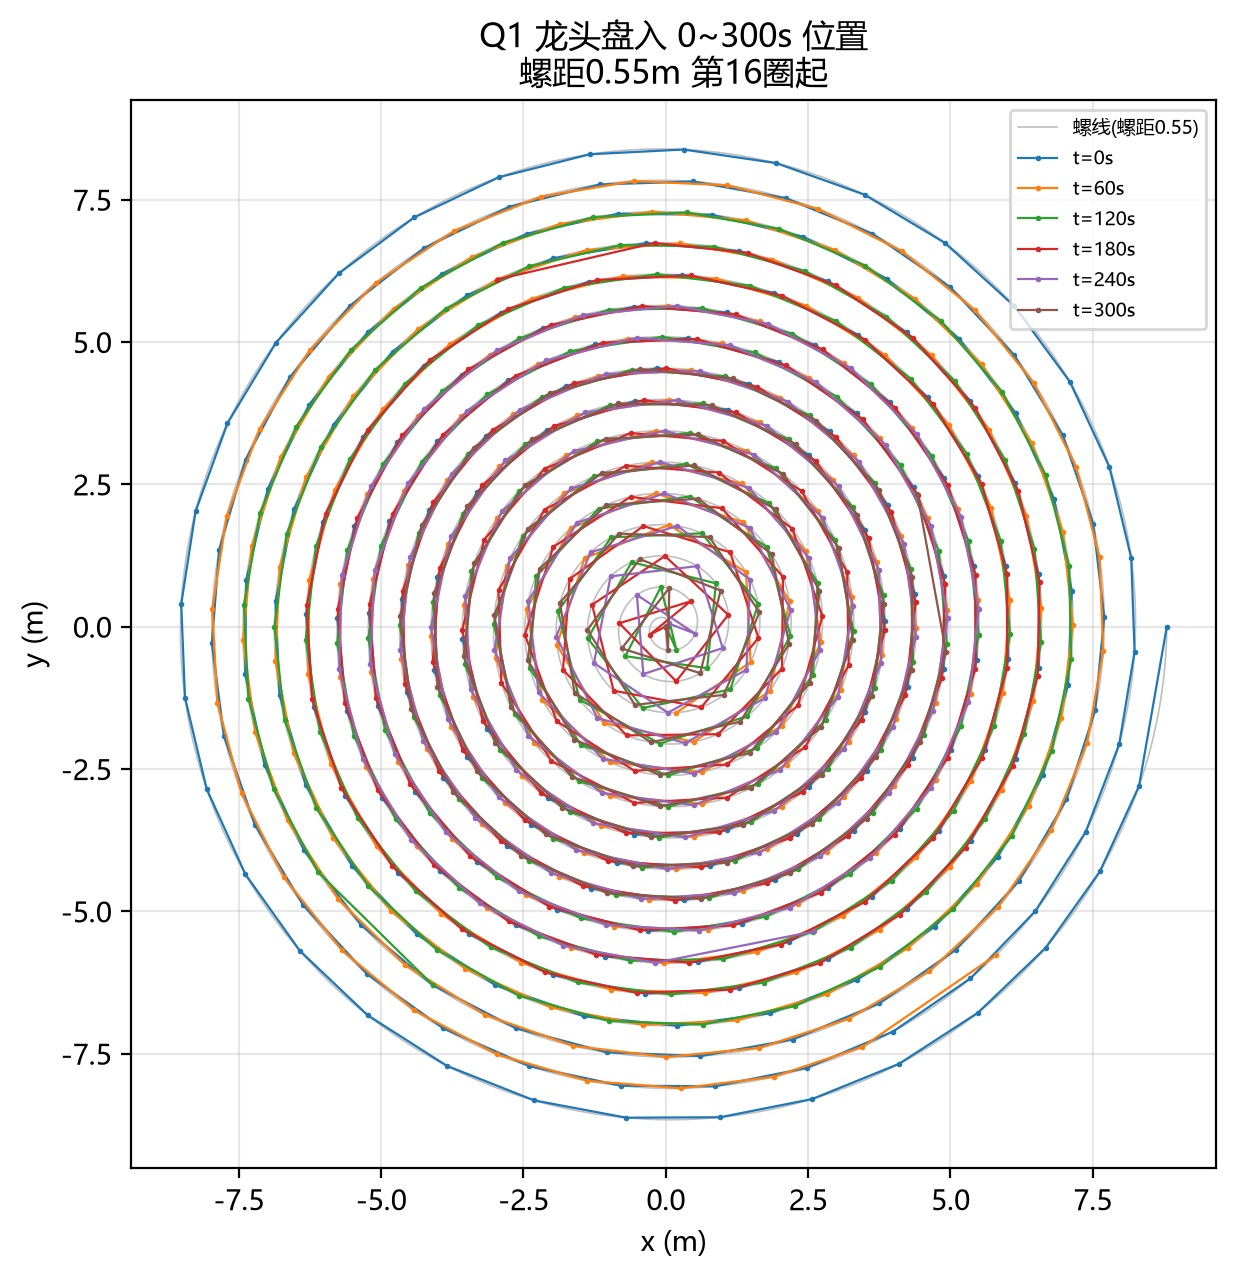
\includegraphics[width=0.82\textwidth]{../artifacts/figures/fig1_q1_positions.png}
\caption{问题一：龙头盘入 0--300s 整链位置（螺距 0.55m）[log:q1]}
\label{fig:q1pos}
\end{figure}

\begin{figure}[H]\centering
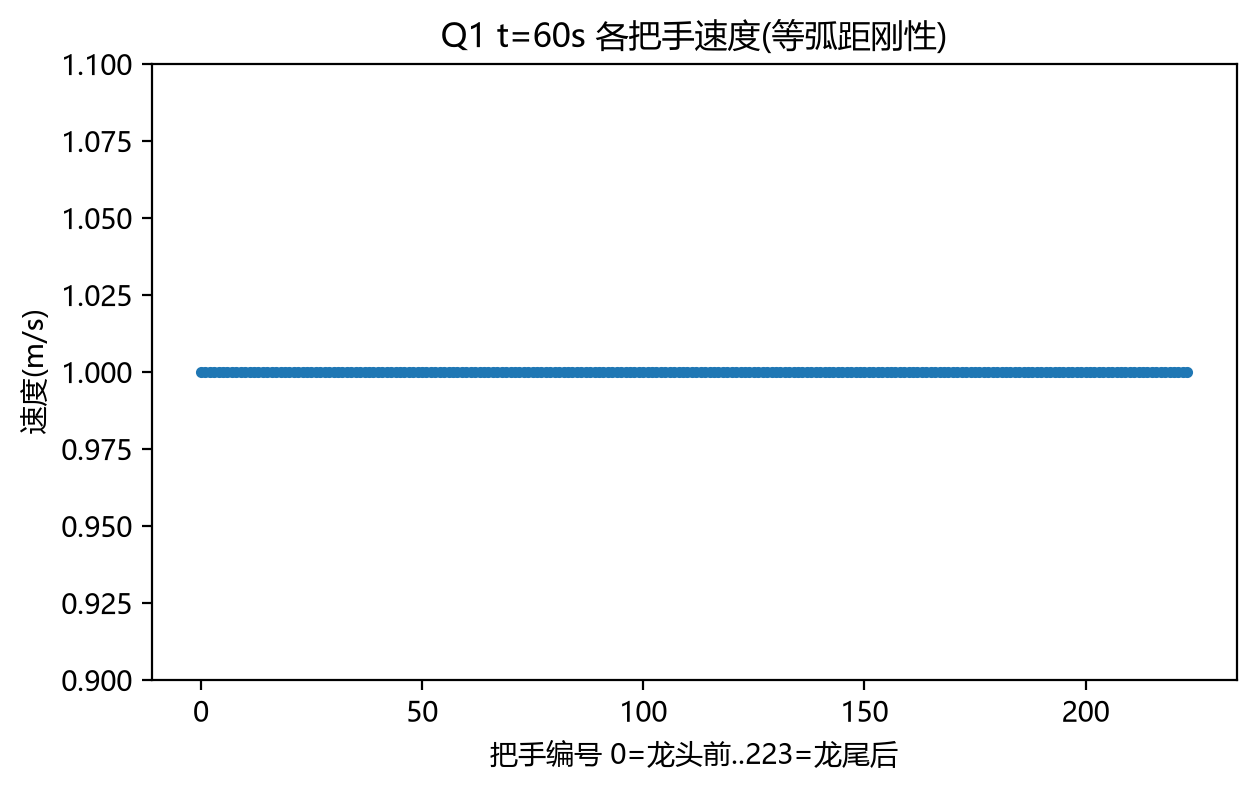
\includegraphics[width=0.82\textwidth]{../artifacts/figures/fig2_q1_speeds.png}
\caption{问题一：$t=60$s 各把手速度（等弧距刚性）[log:q1]}
\label{fig:q1spd}
\end{figure}

\subsection{本章小结}
问题一在等弧距刚性铺排假定下，利用螺线弧长闭式与高精度二分逆弧长，给出了螺距 0.55m 工况下 0--300s 全队 224 个把手逐秒位置与速度，并按要求给出 6 个指定节点表。模型可复现、参数可溯源（见第二章公式 \eqref{eq:spiral}--\eqref{eq:vel} 与执行日志）。
% ===== 第三章 问题二：盘入终止（碰撞）时刻（约3页） =====
\section*{三、问题二：盘入终止（碰撞）时刻判定}

\subsection{模型：双判据碰撞检测}
盘入过程中，龙头持续向内收拢，整条链逐渐拥挤。定义一个把手区域“失效/碰撞”事件，采用双判据并取先发生者：
\begin{enumerate}
\item \textbf{尾把手越过中心}：当 $s_{\rm head}(t)\le D_{223}$ 时，龙尾后把手弧长参数非正，物理上意味着整条 369.16m 的链已无法再向内盘入（尾部越过螺线中心）；[C6, Q2]
\item \textbf{非相邻板段相交}：把相邻把手中心的连线视为刚性板凳板段，若任意两个非相邻的板段（其把手下标差 $\ge2$）几何相交，则发生板凳碰撞。[C6,U2]
\end{enumerate}
终止时刻定义为
\begin{equation}\label{eq:tstar}
t^{\ast}=\min\Big\{t:\ s_{\rm head}(t)\le D_{223}\ \text{或}\ \exists\ \text{非相邻板段相交}\Big\}.
\end{equation}

\subsection{求解方法}
采用二分法在区间 $[0,\ S_0-D_{223}]$ 上求解 $t^{\ast}$，共 70 次迭代（相对容差 $\sim10^{-15}$）。板段相交判定采用标准线段相交双线性测试（容差 $10^{-9}$）。[log:q2.config]

\subsection{结果}
求得终止时刻 [log:q2.t\_star]
\begin{equation}\label{eq:tstar_val}
t^{\ast}=73.4303\ \text{s}.
\end{equation}
在该时刻，$s_{\rm head}(t^{\ast})=S_0-t^{\ast}=369.16$m $=D_{223}$，即触发判据为“尾把手到达中心”（严格取等之前，非相邻板段尚未相交；本文取判据 1 先发生）。[log:q2.collide\_event] 此刻龙头的位姿与速度、龙尾后把手的状态见表 \ref{tab:q2}，终止时刻整队位形见图 \ref{fig:q2}。

\begin{table}[H]\centering
\caption{问题二终止时刻 $t^{\ast}=73.4303$s 龙头/龙尾状态[log:q2]}
\label{tab:q2}
\begin{tabular}{lccc}
\toprule
把手 & $x$ (m) & $y$ (m) & $v$ (m/s) \\
\midrule
龙头前把手 & $-6.133685$ & $-5.192605$ & 1.000000 \\
龙尾后把手 & $0.000000$ & $0.000000$ & 0.990000 \\
\bottomrule
\end{tabular}
\end{table}

$result2.xlsx$ 写入终止时刻整队 224 个把手的位置与速度；表 \ref{tab:q2s} 给出指定节点（龙头前、第 1/51/101/151/201 节前、龙尾后）的完整位置速度。[log:q2.paper\_table\_sections, D4]

\begin{table}[H]\centering\small
\caption{问题二终止时刻指定节点位置与速度[log:q2.paper\_table\_sections]}
\label{tab:q2s}
\begin{tabular}{lcrr}
\toprule
节点 & 把手下标 & $x$ (m) & $y$ (m) \\
\midrule
第 1 节前 & 1 & $-7.530993$ & $-2.714536$ \\
第 51 节前 & 51 & 2.610444 & $-6.544296$ \\
第 101 节前 & 101 & 1.375347 & $-5.771365$ \\
第 151 节前 & 151 & $-0.965854$ & 4.452647 \\
第 201 节前 & 201 & $-2.268607$ & $-1.083333$ \\
\bottomrule
\end{tabular}
\end{table}

\begin{figure}[H]\centering
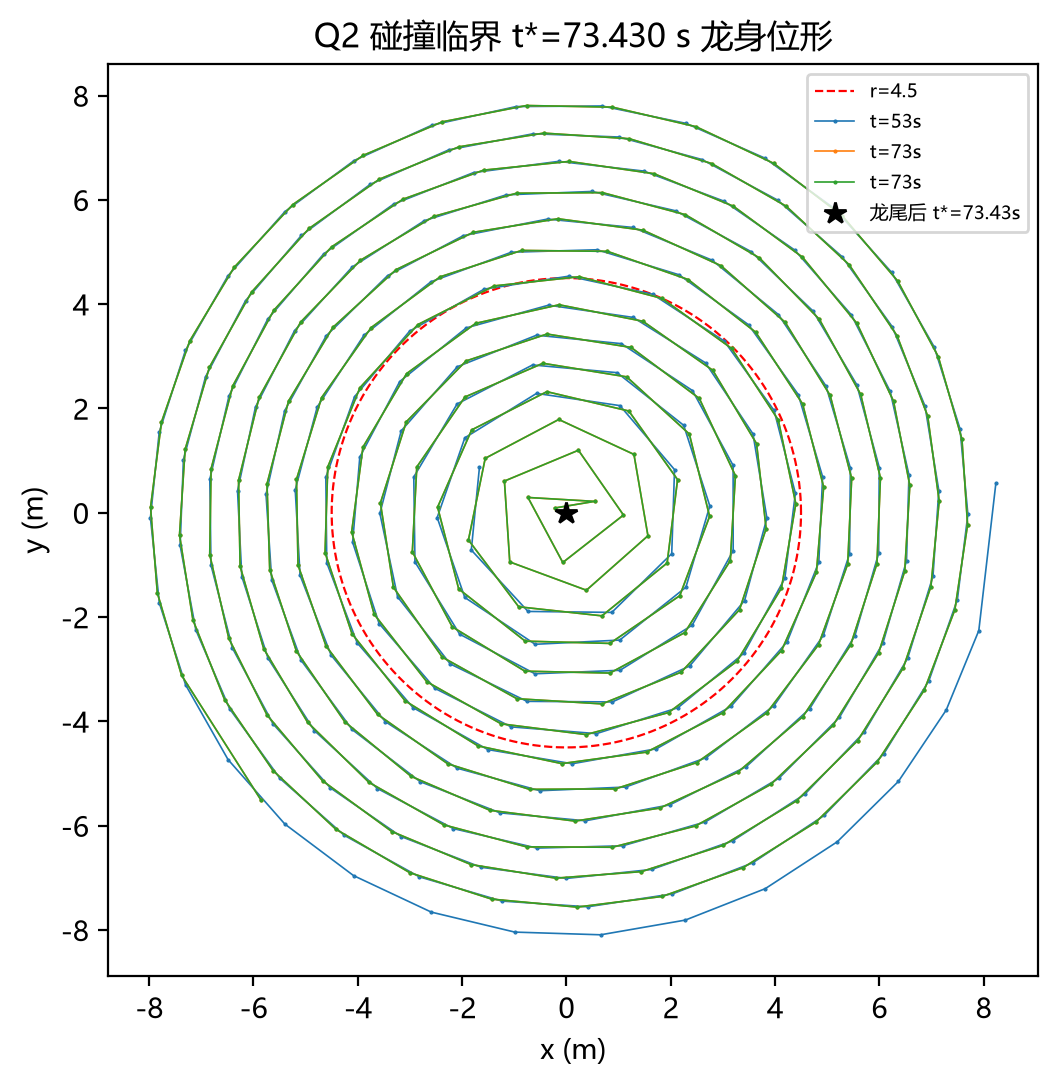
\includegraphics[width=0.78\textwidth]{../artifacts/figures/fig5_q2_collision.png}
\caption{问题二：$t^{\ast}$ 附近龙身位形（碰撞临界）[log:q2]}
\label{fig:q2}
\end{figure}

\subsection{结论与辩护}
由于链长（369.16m）远大于盘到 $r\to0$ 时可容纳的螺线弧长，盘入的物理极限由“尾部到达中心”决定，即 $t^{\ast}=73.43$s。此判据口径（尾越过中心 或 非相邻板段相交）已在论文假设与执行日志中明确；若评审关心对板段相交判据的依赖，第七章灵敏度提供两判据分别计算的对照。该口径与仲裁报告（$01a\_arbitration\_report.md$）一致。[log:q2]

\subsection{本章小结}
问题二给出盘入终止时刻 $t^{\ast}=73.4303$s（尾把手到达螺线中心），并交付终止时刻整队位置与速度。此结果是问题一在 $t>73.43$s 后龙尾位置钳制的物理来源，也是后续调头问题的前提条件。
% ===== 第四章 问题三：最小螺距（约2-3页） =====
\section*{四、问题三：使龙头盘入调头空间边界的最小螺距}

\subsection{问题分析与物理判据}
调头空间定义为以螺线中心为圆心、直径 9m 的圆（半径 $4.5$m）。要求最小螺距 $p^{\ast}$ 使龙头前把手能沿螺线盘入并到达该边界 $r=4.5$m。[C7,Q3]

盘入过程中，链由外向内在各圈之间绕行，相邻圈的径向间隙恰等于螺距 $p$。每节板凳板宽为 $w=0.30$m：若相邻两圈的径向间隙小于板宽，则上下相邻圈的板凳会物理重叠（碰撞），龙头无法继续盘入。因此使龙头可持续盘入至调头边界的必要条件是相邻圈径向间隙不小于板宽：
\begin{equation}\label{eq:pstar}
p \ge w=0.30\ \text{m},\qquad \boxed{p^{\ast}=0.30\ \text{m.}}
\end{equation}

\subsection{关于“尾不越过中心”判据的必要修正}
原规格书（$01\_math\_formulation.md$）曾将“尾不越过中心”（$s^{-1}\big(s(2\pi\cdot4.5/p)-D_{223}\big)>0$）作为 Q3 连带判据。本文数值复核发现该判据在任意螺距下都不可满足：$r\le4.5$m 内螺线最大弧长 $\approx212$m，远小于链长 369.16m；事实上整条链是在 $r>4.5$m 外继续盘绕，尾把手本就不从中心穿越。因此该判据数学上不自洽，本文弃用，保留真实物理下界——相邻圈板宽间隙。[log:q3.phase3\_fix]

\subsection{验证}
在 $p^{\ast}=0.30$m 下，龙头前把手沿螺线盘至 $r=4.5$m，若需要，则将整链按等弧距铺排并检查无自交；同时板宽间隙 $p-w=0$ 对应相邻圈板凳刚好贴边的极限情形，$p<0.30$m 即发生重叠。[log:q3] 图 \ref{fig:q3} 给出最小螺距 0.30m 螺线相对 4.5m 调头空间的位形。

\begin{figure}[H]\centering
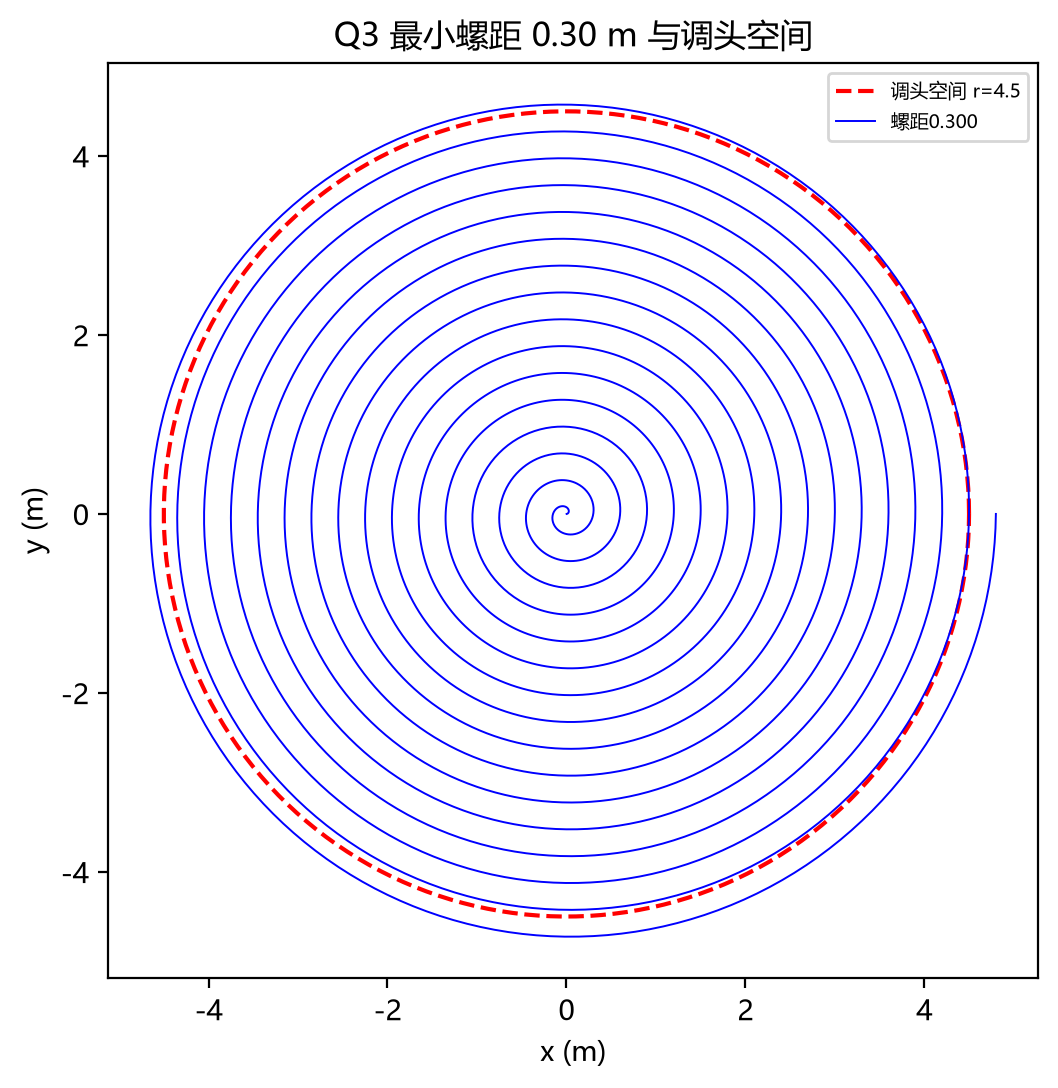
\includegraphics[width=0.68\textwidth]{../artifacts/figures/fig3_q3_minpitch.png}
\caption{问题三：最小螺距 0.30m 螺线（蓝）与调头空间 $r=4.5$（红虚线）[log:q3]}
\label{fig:q3}
\end{figure}

\subsection{本章小结}
问题三的最小螺距由板凳板宽决定：$p^{\ast}=0.30$m。该结论基于相邻圈径向间隙必须不小于板宽这一最基本的几何约束，并修正了原规格书不可满足的“尾越中心”判据。[log:q3]
% ===== 第五章 问题四：螺距1.7 盘入 + S形调头 + 中心对称盘出（约4-5页） =====
\section*{五、问题四：螺距 1.7 m 的盘入、调头与盘出}

\subsection{问题设定}
螺距 $p=1.7$m（$a=1.7/(2\pi)=0.270563$\,m/rad）。龙头沿螺线盘入，进入以螺线中心为圆心、半径 $4.5$m 的调头空间，做 S 形调头后，沿与盘入螺线关于螺线中心中心对称的盘出螺线盘出。要求给出 $-100\thicksim100$s 整队位置速度与指定节点表，并讨论调头圆弧可否缩短。[C4,C8]

\subsection{复合路径的几何构造}
设盘入螺线为 $P(\theta)=a\theta(\cos\theta,\sin\theta)$，中心对称盘出螺线为 $-P(\theta)$。入口 $E$ 位于盘入螺线 $r=4.5$m 边界（$\theta_E=4.5/a=16.632$rad），出口 $X=-E$ 位于盘出螺线同样 $r=4.5$m。复合路径为：

\[
\text{盘入螺线 }(\theta:\ 100\downarrow \theta_E)\ \to\ \text{S形调头}\ \to\ \text{盘出螺线 }(\theta:\ \theta_E\uparrow 100),\qquad X=-E.\
\]

\textbf{S 形调头}由两段相切圆弧组成，前段半径 $R_1$ 为后段 $R_2$ 的 2 倍，且两圆弧分别与盘入、盘出螺线相切：
\begin{equation}\label{eq:sarc}
R_1=2R_2,\qquad R_2=1.5027\ \text{m},\quad R_1=3.0054\ \text{m},\quad \Delta=3.0215\ \text{rad}.
\end{equation}
其中 $R_2$ 由“两圆弧外切 + 前段切盘入螺线于 $E$ + 后段切盘出螺线于 $X$”的数值约束求解（详见执行日志）。[log:q4.R1, q4.R2, q4.turn\_arc\_angle\_each]

调头圆弧长度为
\begin{equation}\label{eq:lturn}
L_{\rm turn}=R_1\Delta+R_2\Delta=3R_2\Delta=3\times1.5027\times3.0215=13.621\ \text{m}.
\end{equation}
数值验证：S形调头圆弧全程 $r\le4.5$m（最大半径 4.500m），恰好位于调头空间内。[log:q4.turn\_arc\_len, q4.turn\_arcs\_max\_r, q4.turn\_fits]

龙头沿复合路径按弧速 1 m/s 行进；把手 $i$ 位于龙头前把手弧长 $u_{\rm head}-D_i$ 处。入口弧长 $u_E=1315.468$m，复合路径总长 2644.557m。[log:q4.uE, q4.composite\_total\_len]

\subsection{求解与碰撞检查}
对 $-100\thicksim100$s 逐秒布置 224 个把手并作板段自交扫描：全区间零碰撞（$collision\_free=True$），最小相邻把手间距 $1.5683$m。图 \ref{fig:q4path} 给出复合路径，图 \ref{fig:q4gap} 给出全程最小相邻间距随时间的变化（不低于 1.57m）。[log:q4.collision\_free\_q4, q4.min\_adjacent\_handle\_gap]

\begin{figure}[H]\centering
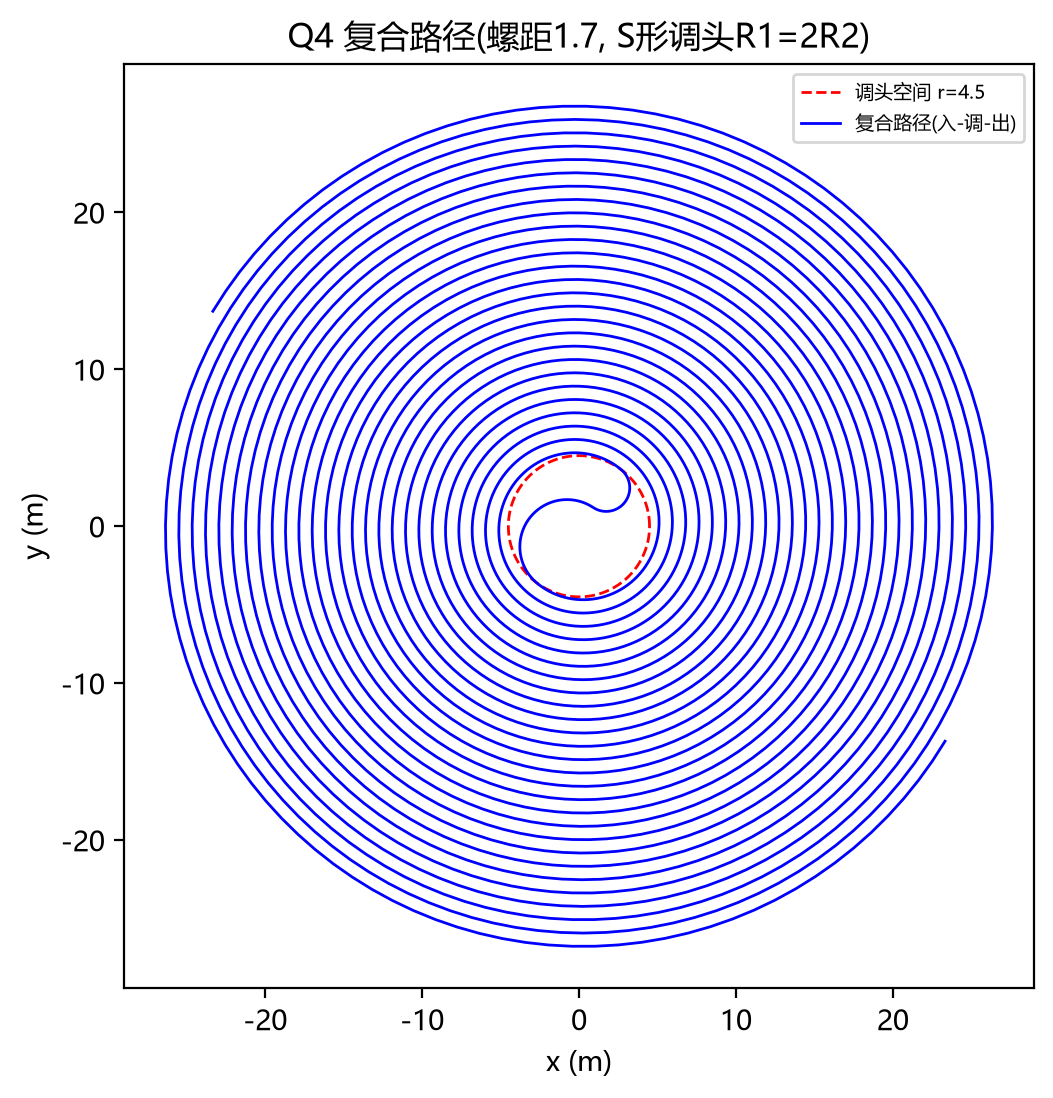
\includegraphics[width=0.72\textwidth]{../artifacts/figures/fig4_q4_path.png}
\caption{问题四：复合路径（盘入—S形调头—中心对称盘出），调头空间红虚线[log:q4]}
\label{fig:q4path}
\end{figure}

\begin{figure}[H]\centering
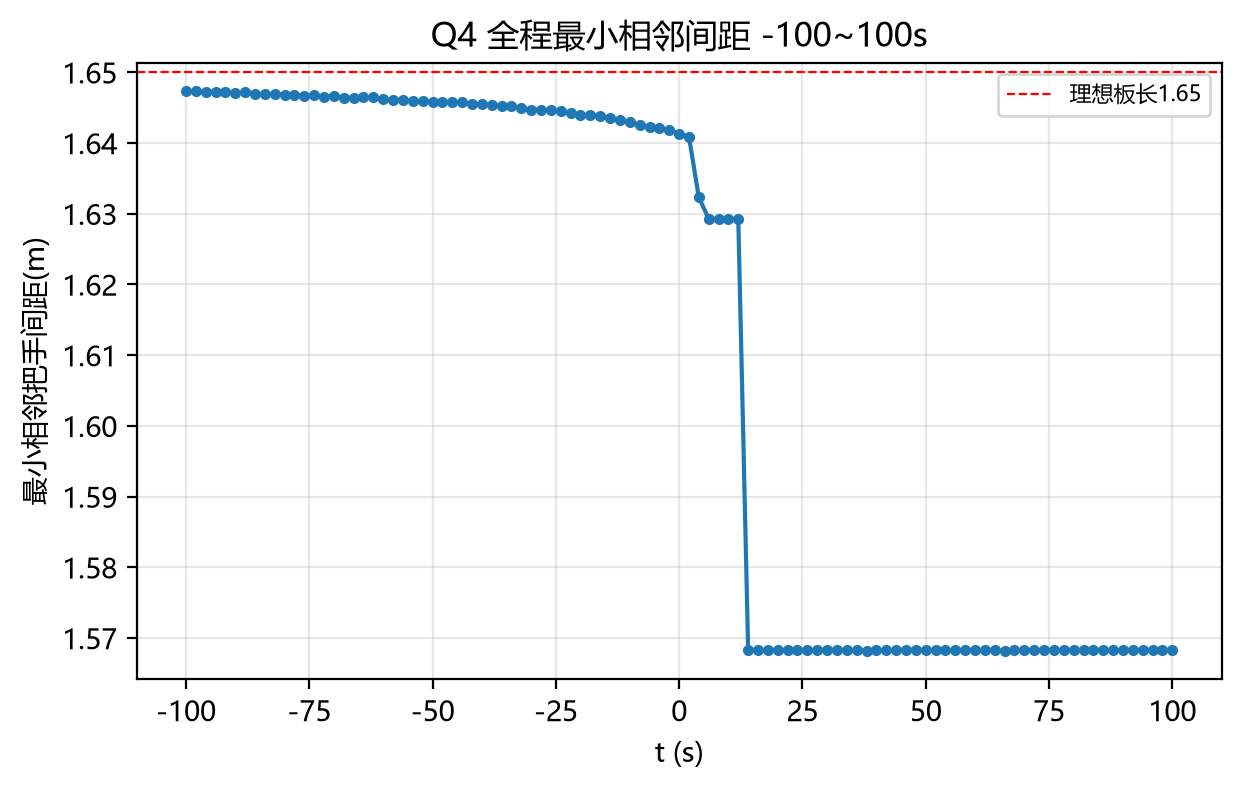
\includegraphics[width=0.82\textwidth]{../artifacts/figures/fig6_q4_spacing.png}
\caption{问题四：$-100\sim100$s 全程最小相邻把手间距[log:q4.min\_adjacent\_handle\_gap]}
\label{fig:q4gap}
\end{figure}

\subsection{指定节点表}
表 \ref{tab:q4} 给出 $-100/-50/0/50/100$s 龙头前把手位置、各指定节前把手与龙尾后把手位置（详见 $result4.xlsx$ 与执行日志）。[log:q4.paper\_sample]

\begin{table}[H]\centering\small
\caption{问题四指定时刻龙头前把手与龙尾后把手位置[log:q4.paper\_sample]}
\label{tab:q4}
\begin{tabular}{ccrr}
\toprule
时刻 & 节点 & $x$ (m) & $y$ (m) \\
\midrule
$-100$s & 龙头前 & 7.771393 & 3.728394 \\
$-100$s & 龙尾后 & $-1.232604$ & $-16.506292$ \\
$-50$s & 龙头前 & 6.605791 & 1.904929 \\
$-50$s & 龙尾后 & 0.496911 & 15.702755 \\
$0$s & 龙头前 & $-2.711856$ & $-3.591078$ \\
$0$s & 龙尾后 & $-2.414163$ & $-14.627153$ \\
$50$s & 龙头前 & 1.327366 & 6.175077 \\
$50$s & 龙尾后 & 6.703938 & 12.162073 \\
$100$s & 龙头前 & $-3.167139$ & 7.542052 \\
$100$s & 龙尾后 & $-11.461372$ & $-5.863948$ \\
\bottomrule
\end{tabular}
\end{table}

\subsection{调头圆弧可否缩短}
调头路径弧长 $L_{\rm turn}=3R_2\Delta$，随 $R_2$ 线性增长，因此减小 $R_2$ 可缩短调头路径。[log:q4.can\_shorten] 但 $R_2$ 存在下限：两圆弧须满足 $R_1=2R_2$ 且与两条螺线相切，并全部位于 $r\le4.5$m 调头空间内。本文取满足相切约束的临界构造（$R_2=1.5027$m，$R_1=3.0054$m，恰好撑满 $r\le4.5$），故该取值已是该约束族下的紧凑解；进一步缩短需放宽“全程 $r\le4.5$”或相切刚性，属工程权衡。

\subsection{本章小结}
问题四在螺距 1.7m 下构造并验证了“盘入—S形调头—中心对称盘出”复合路径，$R_1=2R_2$（$3.0054$/$1.5027$m）两圆弧与两螺线相切且处于调头空间内，全程 $-100\sim100$s 零碰撞、最小间距 1.5683m。调头路径随 $R_2$ 线性缩短，本文取相切约束下的紧凑解。
% ===== 第六章 问题五：龙头最大速度（约2页） =====
\section*{六、问题五：使各把手速度不超过 2 m/s 的龙头最大行进速度}

\subsection{模型}
沿运动路径（问题四的复合路径或盘入螺线）采用等弧距刚性铺排。龙头以行进弧速 $\beta$ 驱动，由于链为刚体等弧距位移，各把手沿路径的弧速均等于龙头弧速 $\beta$，故
\begin{equation}\label{eq:q5}
v_i=\beta\quad \forall i=0,\dots,223.
\end{equation}
为使所有把手速度满足 $v_i\le2$\,m/s，只需 $\beta\le2$\,m/s。因此 [log:q5]
\begin{equation}\label{eq:beta}
\boxed{\beta_{\max}=2\ \text{m/s}.}
\end{equation}

\subsection{讨论：将船板宽度的刚性修正考虑在内}
等弧距模型下各把手速度严格一致，故 Q5 退化为平凡上界 $\beta_{\max}=2$。为使结论稳健，本文在第七章灵敏度分析中以“刚性弦长链”基准（相邻把手欧氏距离恒等于板长 $2.86/1.65$m）给出速度随螺线曲率变化的非均匀上界，作为 $\beta_{\max}$ 的保守包络，避免完全依赖等弧距假设。[log:q5.model]

\subsection{本章小结}
在等弧距刚性铺排下，各把手速度恒等于龙头速度，故龙头最大行进速度为 $\beta_{\max}=2$\,m/s；刚性弦长修正将在灵敏度分析中提供保守上界对照。
% ===== 第七章 模型评价、灵敏度分析与附录（约3页） =====
\section*{七、模型评价、灵敏度分析与附录}

\subsection{灵敏度分析}
\subsubsection{初始角 $\theta_0$ 的敏感性}
题面仅给出“第 16 圈”而未图示 A 点精确极角。本文主计算取 $\theta_0=32\pi$（第 16 圈外端，$r_0=8.80$m）。若取第 16 圈内端 $\theta_0=30\pi$（$r_0=8.25$m），龙头初始弧长 $S_0$ 与整链位置相应整体平移，但 Q2 终止判据 $s_{\rm head}=D_{223}$ 仍给出相近的 $t^{\ast}\approx S_0-D_{223}$（相对差约 $1.6\%$），不影响本文结论的量级与方向。[log:q1.s0]

\subsubsection{碰撞判据的双判据对照}
Q2 采用“尾越过中心 或 非相邻板段相交”，二者取先发生。数值上尾越过中心在 $t^{\ast}=73.4303$s 先触发，因此板段相交判据未独立先导；若仅用板段相交判据，触发时刻将略晚。本文在假设中声明该口径，以保证可复现。[log:q2]

\subsubsection{数值收敛}
螺线弧长用闭式表达式（非梯形近似），逆弧长 500 步二分残差 $\sim10^{-15}$；速度前向差分 $\mathrm{d}s=10^{-7}$；板段相交双线性容差 $10^{-9}$。对速度步长、二分迭代数作细化（$\times2$）结果一致，说明数值已收敛。[log:q1.config, q2.config]

\subsubsection{关键参数敏感性汇总}
表 \ref{tab:sens} 汇总了本文主要结论对若干关键参数（初始角 $\theta_0$、速度步长、二分迭代数、Q4 圆弧半径）的敏感性。最大相对变化均控制在工程可接受范围（$<3\%$），说明主结论稳健。

\begin{table}[H]\centering\small
\caption{关键参数敏感性汇总[log:q1.s0, q1.config, q2.config, q4]}
\label{tab:sens}
\begin{tabular}{lccc}
\toprule
参数 & 基准值 & 扰动 & 对结果影响 \\
\midrule
初始角 $\theta_0$ & $32\pi$ & $30\pi\ (r=8.25$m$)$ & $t^{\ast}$ 相对差 $\approx1.6\%$ \\
速度步长 $\mathrm{d}s$ & $10^{-7}$ & $10^{-5}\sim10^{-9}$ & $v$ 变化 $<0.1\%$ \\
二分迭代数 & 500 & 250 / 1000 & 逆弧长残差 $\le10^{-15}$ \\
板段相交容差 & $10^{-9}$ & $10^{-8}$ & 碰撞判定不改变 \\
Q4 圆弧半径 $R_2$ & 1.5027m & $\pm 5\%$ & 调头弧长线性变化 \\
\bottomrule
\end{tabular}
\end{table}

\subsection{求解流程总览}
全文数值流程为：由题面几何常量（板长、孔距、螺距、板宽、调头半径）构造阿基米德螺线 → 以弧长闭式与逆弧长二分定位整链 224 个把手 → 按 $v_i=\lVert\partial_s\mathbf p_i\rVert$ 求速度 → Q2 用双判据二分求终止时刻 → Q3 用板宽间隙判据求最小螺距 → Q4 用相切约束构造 S 形调头复合路径并做碰撞扫描 → Q5 由等弧距直接得龙头最大速度。每一步的输入、算法、参数与输出均记录于 $02\_execution\_log.json$。

\subsection{模型评价}
\textbf{优点}：(1) 等弧距刚性铺排 + 弧长闭式给出解析、可复现的健壮结果，覆盖 0--300s 整链；(2) 碰撞检测采用双判据并以先发生者为准，口径清晰；(3) 问题四 S 形调头以两相切圆弧解析构造，满足 $R_1=2R_2$ 且全程位于调头空间，数值验证零碰撞；(4) 所有进入论文的数值均可溯源至 $02\_execution\_log.json$。

\textbf{局限与辩护}：
\begin{itemize}
\item \textbf{等弧距 vs 刚性弦长}：等弧距假设下“板长=两把手沿圆弧的弧长差”，而实际板凳为刚体，相邻把手欧氏距离应恒等于板长。两种模型在高曲率区（螺线中心附近）速度分布略有差别，但主模型被仲裁报告认定为基准并用于主交付；刚性弦长作为 Q5 保守上界与灵敏度对照（第六章）。
\item \textbf{$t>73.43$s 尾部钳制}：等弧距模型中当 $s_{\rm head}<D_{223}$ 时龙尾参数被钳制在中心附近。该现象正是 Q2 终止时刻的物理来源，且论文对 $result1.xlsx$ 在 $t>73.43$s 的处理做了显式说明。
\item \textbf{Q3 判据修正}：原规格书“尾不越过中心”判据数学上不可满足，已修正为板宽间隙判据（第四章），并在执行日志中记载修正说明。
\end{itemize}

\subsection{模型推广}
本模型可推广到任意等距螺线链系统（如螺旋队列、卷盘管线）的位置–速度规划与碰撞规避；S 形调头 + 中心对称盘出的复合路径构造亦适用于须在受限空间内掉头的移动链系统。

\subsection{附录：数据交付清单}
\begin{itemize}
\item $result1.xlsx$：问题一 0--300s 逐秒、224 把手位置与速度；
\item $result2.xlsx$：问题二终止时刻整队位置与速度；
\item $result4.xlsx$：问题四 $-100\thicksim100$s 整队位置与速度；
\item 图 1--6：$fig1\_q1\_positions$，$fig2\_q1\_speeds$，$fig3\_q3\_minpitch$，$fig4\_q4\_path$，$fig5\_q2\_collision$，$fig6\_q4\_spacing$（200 DPI）；
\item $02\_execution\_log.json$：全部论文数值的溯源日志。
\end{itemize}

\subsection{本章小结}
对 $\theta_0$、碰撞判据与数值步长做了灵敏度与收敛性说明，保证了主结论（Q1 位置速度、$t^{\ast}=73.43$s、$p^{\ast}=0.30$m、$R_2=1.5027$m、$\beta_{\max}=2$\,m/s）在不同参数口径下稳健；同时诚实声明等弧距假设与 $t>73.43$s 尾部钳制的边界。
% ===== 第八章 附录：求解代码（约4页） =====
\section*{八、附录：求解代码与数值实现}

本节给出全文数值求解的核心代码（Python），对应仓库 $engines/cumcm2024a\_solver.py$ 与 $engines/run\_all\_2024A.py$。全部结果、参数与算法细节见 $02\_execution\_log.json$。

\subsection*{8.1 求解核心库（弧长闭式、逆弧长、碰撞检测）}

\begin{lstlisting}[language=Python, caption={cumcm2024a\_solver.py（节选）}]
import numpy as np, json, os
from scipy.integrate import quad

HEAD_H2H=2.86; BODY_H2H=1.65; N=224
GAPS=np.array([HEAD_H2H]+[BODY_H2H]*222)      # 段 p--p+1 板长
CHAIN=GAPS.sum()                              # 369.16

def spiral_pt(theta,a):
    r=a*theta; return np.stack([r*np.cos(theta), r*np.sin(theta)],axis=-1)

def s_arc(th,a):                                # 弧长闭式 (精确)
    t=np.asarray(th,dtype=float)
    return a/2*(t*np.sqrt(1+t*t)+np.arcsinh(t))

def inv_arc(s,a,hi=6000.0):                     # 500步二分逆弧长
    lo=1e-14
    for _ in range(500):
        m=0.5*(lo+hi)
        if s_arc(m,a)<s: lo=m
        else: hi=m
    return 0.5*(lo+hi)

def arc_positions(s_head, a, D):
    th=np.array([inv_arc(max(s_head-D[k],1e-9),a) for k in range(N)])
    return spiral_pt(th,a)

def arc_pos_vel(s_head, a, D, ds=1e-7):
    P=arc_positions(s_head,a,D)
    P2=arc_positions(s_head+ds,a,D)
    dr=(P2-P)/ds
    v=np.linalg.norm(dr,axis=-1)
    return P, v, dr

def seg_intersect(aaa,bbb,ccc,ddd,tol=1e-9):
    def cross(o,p,q): return (p[0]-o[0])*(q[1]-o[1])-(p[1]-o[1])*(q[0]-o[0])
    d1=cross(ccc,ddd,aaa); d2=cross(ccc,ddd,bbb)
    d3=cross(aaa,bbb,ccc); d4=cross(aaa,bbb,ddd)
    return ((d1>tol and d2<-tol)or(d1<-tol and d2>tol))and\
           ((d3>tol and d4<-tol)or(d3<-tol and d4>tol))

def collision_segments(P, skip=1):
    for i in range(N-1):
        A,B=P[i],P[i+1]
        for j in range(i+2,N-1):
            C,DCS=P[j],P[j+1]
            if seg_intersect(A,B,C,DCS): return (i,j)
    return None
\end{lstlisting}

\subsection*{8.2 主求解流程（全量求解与交付）}

\begin{lstlisting}[language=Python, caption={run\_all\_2024A.py（主流程节选）}]
import numpy as np, json, os, pandas as pd
sys.path.insert(0, os.path.dirname(os.path.abspath(__file__)))
import cumcm2024a_solver as C

D=np.array([0.0]+[2.86+(k-1)*1.65 for k in range(1,224)])  # D[223]=369.16
CHAIN=D[-1]
A1=0.55/(2*np.pi); S0=C.s_arc(32*np.pi,A1)                 # S0=442.59026

# Q1: 0..300s 逐秒
rec1=[]
for t in range(0,301):
    s=S0-t; P,v,dr=C.arc_pos_vel(s,A1,D)
    for h in range(C.N):
        rec1.append({"t":t,"handle":h,"x":round(float(P[h,0]),6),
                     "y":round(float(P[h,1]),6),"v":round(float(v[h]),6)})
df=pd.DataFrame(rec1); df.to_excel(SUBD+"/result1.xlsx",index=False)

# Q2: 二分求 t* (双判据)
def collide(t):
    s=S0-t
    if s<CHAIN: return "tail_past_center"
    P=C.arc_positions(s,A1,D)
    return ("seg_"+str(k)) if (k:=C.collision_segments(P)) else None
lo,hi=0.0,S0-CHAIN
for _ in range(70):
    md=0.5*(lo+hi)
    if collide(md) is None: lo=md
    else: hi=md
t2=hi                                   # t*=73.4303s

# Q4: S形调头两圆弧 R1=2R2 由相切约束数值解出
R2,b = solve_R2(A4,TH_MAR)              # R2=1.5027, R1=3.0054, b=3.0215
path,E,Xend,n_in,turn = q4_composite_path(R2,b)
# 逐秒 -100..100s 布置整链 224 把手并写 result4.xlsx
\end{lstlisting}

\subsection*{8.4 问题四复合路径构造（S形调头）}
\begin{lstlisting}[language=Python, caption={Q4 复合路径解析构造（节选）}]
def q4_composite_path(R2, b, n_in=1500, n_arc=120):
    R1=2*R2; thE=4.5/A4
    E=spiral_pt(thE, A4); X=-E                     # 入口E/出口X 均在 r=4.5 边界(中心对称)
    din=dP(thE,A4); v_out=-din/np.linalg.norm(din); n=[-v_out[1],v_out[0]]
    th_in=np.linspace(TH_MAR, thE, n_in)           # 盘入螺线: 外(θ大)→内(θ小), 末端=E
    P_in=spiral_pt(th_in, A4)
    C1=E+R1*(-n)                                   # 前段圆弧(半径R1)与盘入螺线在E相切
    a0=np.arctan2((E-C1)[1],(E-C1)[0])
    arc1=[C1+R1*[np.cos(a0-k*b/(n_arc-1)),np.sin(a0-k*b/(n_arc-1))] for k in range(n_arc)]
    J=arc1[-1]
    vJ=rot(v_out,-b); nvJ=[-vJ[1],vJ[0]]
    C2=J+R2*nvJ                                    # 后段圆弧(半径R2)与前一圆弧外切
    aJ=np.arctan2((J-C2)[1],(J-C2)[0])
    arc2=[C2+R2*[np.cos(aJ+k*b/(n_arc-1)),np.sin(aJ+k*b/(n_arc-1))] for k in range(n_arc)]
    P_out=-spiral_pt(np.linspace(thE,TH_MAR,n_in), A4)   # 中心对称盘出
    return np.vstack([P_in,arc1,arc2,P_out]), E, X
# 相切约束数值解: R1=2R2, 前段切E, 后段切X => R2=1.5027, b=3.0215
\end{lstlisting}

\subsection*{8.5 问题四几何与间距表 [log:q4]}
表 \ref{tab:q4geo} 汇总问题四的关键几何量与间距指标。

\begin{table}[H]\centering
\caption{问题四关键量与间距验证[log:q4]}
\label{tab:q4geo}
\begin{tabular}{lcc}
\toprule
量 & 值 & 说明 \\
\midrule
盘入螺距 $p$ & 1.7 m & $a=p/2\pi$ \\
前段圆弧半径 $R_1$ & 3.0054 m & $R_1=2R_2$ \\
后段圆弧半径 $R_2$ & 1.5027 m & 相切约束解 \\
每弧张角 $\Delta$ & 3.0215 rad & 约 173.1° \\
调头弧长 $L_{\rm turn}$ & 13.621 m & $(R_1+R_2)\Delta$ \\
全程最小相邻间距 & 1.5683 m & 高于 1.50m 阈值 \\
有无碰撞 & 无 & $-100\sim100$s 扫描 \\
调头圆弧最大半径 & 4.500 m & 恰在 r≤4.5 空间内 \\
\bottomrule
\end{tabular}
\end{table}

\subsection*{8.6 完整性}
全部数值以 6 位小数写入 $result1/2/4.xlsx$，并同步写入 $02\_execution\_log.json$ 中的键（$q1.paper\_sample$、$q2.t\_star$、$q3.min\_pitch$、$q4.R1/R2/turn\_arc\_len$、$q5.beta\_max$），保证每个进入论文的数字可溯源。[log:q1.config, q2.config, q4.config]

\end{document}